
        \documentclass[spanish, 11pt]{exam}

        %These tell TeX which packages to use.
        \usepackage{array,epsfig}
        \usepackage{amsmath, textcomp}
        \usepackage{amsfonts}
        \usepackage{amssymb}
        \usepackage{amsxtra}
        \usepackage{amsthm}
        \usepackage{mathrsfs}
        \usepackage{color}
        \usepackage{multicol, xparse}
        \usepackage{verbatim}


        \usepackage[utf8]{inputenc}
        \usepackage[spanish]{babel}
        \usepackage{eurosym}

        \usepackage{graphicx}
        \graphicspath{{../img/}}
        \usepackage{pgf}
        
        \usepackage{pgfplots}
        \usetikzlibrary{math}
        \pgfplotsset{compat=1.15}
        \usepackage{xfp}

        \printanswers
        \nopointsinmargin
        \pointformat{}

        %Pagination stuff.
        %\setlength{\topmargin}{-.3 in}
        %\setlength{\oddsidemargin}{0in}
        %\setlength{\evensidemargin}{0in}
        %\setlength{\textheight}{9.in}
        %\setlength{\textwidth}{6.5in}
        %\pagestyle{empty}

        \let\multicolmulticols\multicols
        \let\endmulticolmulticols\endmulticols
        \RenewDocumentEnvironment{multicols}{mO{}}
         {%
          \ifnum#1=1
            #2%
          \else % More than 1 column
            \multicolmulticols{#1}[#2]
          \fi
         }
         {%
          \ifnum#1=1
          \else % More than 1 column
            \endmulticolmulticols
          \fi
         }
        \renewcommand{\solutiontitle}{\noindent\textbf{Sol:}\enspace}

        \newcommand{\samedir}{\mathbin{\!/\mkern-5mu/\!}}

        \newcommand{\class}{2º Bachillerato CCSS}
        \newcommand{\examdate}{\today}

        \newcommand{\tipo}{A}


        \newcommand{\timelimit}{50 minutos}



        \pagestyle{head}
        \firstpageheader{
\includegraphics[width=0.2\columnwidth]{header_left}}{\textbf{Departamento de Matemáticas\linebreak \class}\linebreak \examnum}{
\includegraphics[width=0.1\columnwidth]{header_right}}
        \runningheader{\class}{\examnum}{Página \thepage\ of \numpages}
        \runningheadrule

        \newcommand{\examnum}{Intervalos de confianza}
        \begin{document}
        \begin{questions}
        \question p71e01-Una muestra aleatoria de 36 personas, empleadas en una gran industria, da el número medio de días al año
que faltan al trabajo es $\overline{x} = 12$ con $s = 4$.
a) Dar una estimación puntual de $\mu$.
b) Tomando un nivel del 99\% dar el intervalo de confianza de $\mu$.
c) Tomando un nivel del 95\% dar el intervalo de confianza de $\mu$. \begin{solution}   a) $\mu\approx 12$ \\ b) Calculamos el intervalo de confianza para la media, sabiendo que la media muestral es: 12, la desviación típica: 4, tamaño de la muestra: 36 y el grado de confianza: 99.0\%. \\ \\ Valor crítico: \\ $\alpha=1-0.99=0.01\to \frac{\alpha}{2}=0.005$ \\ \\ $P(Z>z_{\alpha/2})=0.005\to P(Z<z_{\alpha/2})=0.995 \to z_{\alpha/2} =2.5758$ \\ 
    \begin{tikzpicture}[scale=0.8]
    \pgfmathdeclarefunction{gauss}{2}{\pgfmathparse{1/(#2*sqrt(2*pi))*exp(-((x-#1)^2)/(2*#2^2))}}
    \tikzmath{\conf = 0.99; \crit= 2.5758; \a=0.005);}
    \begin{axis}[no markers, domain=-5:5, samples=100, axis lines=left, height=5cm, width=12cm, xtick={0,\crit}, ytick=\empty, xticklabels = {$0$, $z_{\frac{\alpha}{2}}=\crit$},enlargelimits=false, clip=false, axis on top]
      \addplot [fill=cyan!20, draw=none, domain=-\crit:\crit] {gauss(0,1)} \closedcycle;
      \addplot [very thick,cyan!50!black] {gauss(0,1)};
    \end{axis}
    \node[] at (5.2,1.5) {$\conf$};	
    \draw[-]   (\crit+6.5,1)node[right]{$\a$}  --  (\crit+5.6,0.1) ;
    \end{tikzpicture} \\
    Error cometido: \\ $E=z_{\alpha/2}\cdot \frac{\sigma}{\sqrt{n}} \to E=2.5758\cdot \frac{4}{6.0}=1.7172$ \\ Por tanto el intervalo de confianza será: \\$\left(\overline{x} - E , \overline{x} + E \right)=\left(12 - 1.7172 , 12 + 1.7172 \right)=\left(10.2828, 13.7172 \right)$ \\  \\ 
    \begin{tikzpicture}[scale=0.4]
      \tikzmath{\a = -10; \b = 10; \aa = \a -1; \bb = \b + 1 ; \dist = \b - \a; \med = (\a + \b)/2;}
      \draw[very thick] (\a,0) -- (\b,0);
      \path [draw=black, fill=white] (\b,0) circle (2pt);
      \path [draw=black, fill=white] (\a,0.0) circle (2pt);
      \draw[latex-latex] (\a - 1.5,0) -- (\b + 1.5,0) ;
      \draw[shift={(\a,0)},color=black] (0pt,3pt) -- (0pt,-3pt);
      \draw[shift={(\a,0)},color=black] (0pt,0pt) -- (0pt,-3pt) node[below] {$10.2828$};
      \draw[shift={(\med,0)},color=black] (0pt,3pt) -- (0pt,-3pt);
      \draw[shift={(\med,0)},color=black] (0pt,0pt) -- (0pt,-3pt) node[below] {$12$};
      \draw[shift={(\b,0)},color=black] (0pt,3pt) -- (0pt,-3pt);
      \draw[shift={(\b,0)},color=black] (0pt,0pt) -- (0pt,-3pt) node[below] {$13.7172$};
      \draw[decorate,decoration={brace}, thick](\med,0.2)--(\b,0.2) node[above, midway] {$E=1.7172$}; 
    \end{tikzpicture} \\
    \\ c) Calculamos el intervalo de confianza para la media, sabiendo que la media muestral es: 12, la desviación típica: 4, tamaño de la muestra: 36 y el grado de confianza: 95.0\%. \\ \\ Valor crítico: \\ $\alpha=1-0.95=0.05\to \frac{\alpha}{2}=0.025$ \\ \\ $P(Z>z_{\alpha/2})=0.025\to P(Z<z_{\alpha/2})=0.975 \to z_{\alpha/2} =1.96$ \\ 
    \begin{tikzpicture}[scale=0.8]
    \pgfmathdeclarefunction{gauss}{2}{\pgfmathparse{1/(#2*sqrt(2*pi))*exp(-((x-#1)^2)/(2*#2^2))}}
    \tikzmath{\conf = 0.95; \crit= 1.96; \a=0.025);}
    \begin{axis}[no markers, domain=-5:5, samples=100, axis lines=left, height=5cm, width=12cm, xtick={0,\crit}, ytick=\empty, xticklabels = {$0$, $z_{\frac{\alpha}{2}}=\crit$},enlargelimits=false, clip=false, axis on top]
      \addplot [fill=cyan!20, draw=none, domain=-\crit:\crit] {gauss(0,1)} \closedcycle;
      \addplot [very thick,cyan!50!black] {gauss(0,1)};
    \end{axis}
    \node[] at (5.2,1.5) {$\conf$};	
    \draw[-]   (\crit+6.5,1)node[right]{$\a$}  --  (\crit+5.6,0.1) ;
    \end{tikzpicture} \\
    Error cometido: \\ $E=z_{\alpha/2}\cdot \frac{\sigma}{\sqrt{n}} \to E=1.96\cdot \frac{4}{6.0}=1.3067$ \\ Por tanto el intervalo de confianza será: \\$\left(\overline{x} - E , \overline{x} + E \right)=\left(12 - 1.3067 , 12 + 1.3067 \right)=\left(10.6933, 13.3067 \right)$ \\  \\ 
    \begin{tikzpicture}[scale=0.4]
      \tikzmath{\a = -10; \b = 10; \aa = \a -1; \bb = \b + 1 ; \dist = \b - \a; \med = (\a + \b)/2;}
      \draw[very thick] (\a,0) -- (\b,0);
      \path [draw=black, fill=white] (\b,0) circle (2pt);
      \path [draw=black, fill=white] (\a,0.0) circle (2pt);
      \draw[latex-latex] (\a - 1.5,0) -- (\b + 1.5,0) ;
      \draw[shift={(\a,0)},color=black] (0pt,3pt) -- (0pt,-3pt);
      \draw[shift={(\a,0)},color=black] (0pt,0pt) -- (0pt,-3pt) node[below] {$10.6933$};
      \draw[shift={(\med,0)},color=black] (0pt,3pt) -- (0pt,-3pt);
      \draw[shift={(\med,0)},color=black] (0pt,0pt) -- (0pt,-3pt) node[below] {$12$};
      \draw[shift={(\b,0)},color=black] (0pt,3pt) -- (0pt,-3pt);
      \draw[shift={(\b,0)},color=black] (0pt,0pt) -- (0pt,-3pt) node[below] {$13.3067$};
      \draw[decorate,decoration={brace}, thick](\med,0.2)--(\b,0.2) node[above, midway] {$E=1.3067$}; 
    \end{tikzpicture} \\
       \end{solution}\question p71e02- Cuál debe ser el tamaño de una muestra si se quiere estimar el gasto medio de una familia en electricidad,
mensualmente, con un error menor de 1.500 pesetas y el 95/% como nivel de confianza, sabiendo que el gasto
medio en 1999 era de 13.300 ptas. con una desviación de 1.200 ptas. \begin{solution}   $\alpha=1-0.95=0.05\to \frac{\alpha}{2}=0.025$ \\ \\ Valor crítico: \\ $P(Z>z_{\alpha/2})=0.025\to P(Z<z_{\alpha/2})=0.975 \to z_{\alpha/2} =1.96$ \\ 
    \begin{tikzpicture}[scale=0.8]
    \pgfmathdeclarefunction{gauss}{2}{\pgfmathparse{1/(#2*sqrt(2*pi))*exp(-((x-#1)^2)/(2*#2^2))}}
    \tikzmath{\conf = 0.95; \crit= 1.96; \a=0.025);}
    \begin{axis}[no markers, domain=-5:5, samples=100, axis lines=left, height=5cm, width=12cm, xtick={0,\crit}, ytick=\empty, xticklabels = {$0$, $z_{\frac{\alpha}{2}}=\crit$},enlargelimits=false, clip=false, axis on top]
      \addplot [fill=cyan!20, draw=none, domain=-\crit:\crit] {gauss(0,1)} \closedcycle;
      \addplot [very thick,cyan!50!black] {gauss(0,1)};
    \end{axis}
    \node[] at (5.2,1.5) {$\conf$};	
    \draw[-]   (\crit+6.5,1)node[right]{$\a$}  --  (\crit+5.6,0.1) ;
    \end{tikzpicture} \\
    Error cometido: \\ $E=z_{\alpha/2}\cdot \frac{\sigma}{\sqrt{n}} \to n =\frac{\sigma^2 \cdot z_{\alpha / 2}^2}{E^2} \to n \geq3$ \\    \end{solution}\question p71e03- Una muestra aleatoria de 100 bombillas producidas por una determinada fábrica, tiene una vida media de
1.280 horas con una desviación típica de 140 horas:
i) Estimar la duración media de las bombillas fabricas por esa fábrica.
ii) Dar el intervalo de confianza, a un nivel del 0,95 de la estimación anterior. \begin{solution}   i) $\mu\approx 1280$ \\ ii) Calculamos el intervalo de confianza para la media, sabiendo que la media muestral es: 1280, la desviación típica: 140, tamaño de la muestra: 100 y el grado de confianza: 95.0\%. \\ \\ Valor crítico: \\ $\alpha=1-0.95=0.05\to \frac{\alpha}{2}=0.025$ \\ \\ $P(Z>z_{\alpha/2})=0.025\to P(Z<z_{\alpha/2})=0.975 \to z_{\alpha/2} =1.96$ \\ 
    \begin{tikzpicture}[scale=0.8]
    \pgfmathdeclarefunction{gauss}{2}{\pgfmathparse{1/(#2*sqrt(2*pi))*exp(-((x-#1)^2)/(2*#2^2))}}
    \tikzmath{\conf = 0.95; \crit= 1.96; \a=0.025);}
    \begin{axis}[no markers, domain=-5:5, samples=100, axis lines=left, height=5cm, width=12cm, xtick={0,\crit}, ytick=\empty, xticklabels = {$0$, $z_{\frac{\alpha}{2}}=\crit$},enlargelimits=false, clip=false, axis on top]
      \addplot [fill=cyan!20, draw=none, domain=-\crit:\crit] {gauss(0,1)} \closedcycle;
      \addplot [very thick,cyan!50!black] {gauss(0,1)};
    \end{axis}
    \node[] at (5.2,1.5) {$\conf$};	
    \draw[-]   (\crit+6.5,1)node[right]{$\a$}  --  (\crit+5.6,0.1) ;
    \end{tikzpicture} \\
    Error cometido: \\ $E=z_{\alpha/2}\cdot \frac{\sigma}{\sqrt{n}} \to E=1.96\cdot \frac{140}{10.0}=27.44$ \\ Por tanto el intervalo de confianza será: \\$\left(\overline{x} - E , \overline{x} + E \right)=\left(1280 - 27.44 , 1280 + 27.44 \right)=\left(1252.56, 1307.44 \right)$ \\  \\ 
    \begin{tikzpicture}[scale=0.4]
      \tikzmath{\a = -10; \b = 10; \aa = \a -1; \bb = \b + 1 ; \dist = \b - \a; \med = (\a + \b)/2;}
      \draw[very thick] (\a,0) -- (\b,0);
      \path [draw=black, fill=white] (\b,0) circle (2pt);
      \path [draw=black, fill=white] (\a,0.0) circle (2pt);
      \draw[latex-latex] (\a - 1.5,0) -- (\b + 1.5,0) ;
      \draw[shift={(\a,0)},color=black] (0pt,3pt) -- (0pt,-3pt);
      \draw[shift={(\a,0)},color=black] (0pt,0pt) -- (0pt,-3pt) node[below] {$1252.56$};
      \draw[shift={(\med,0)},color=black] (0pt,3pt) -- (0pt,-3pt);
      \draw[shift={(\med,0)},color=black] (0pt,0pt) -- (0pt,-3pt) node[below] {$1280$};
      \draw[shift={(\b,0)},color=black] (0pt,3pt) -- (0pt,-3pt);
      \draw[shift={(\b,0)},color=black] (0pt,0pt) -- (0pt,-3pt) node[below] {$1307.44$};
      \draw[decorate,decoration={brace}, thick](\med,0.2)--(\b,0.2) node[above, midway] {$E=27.44$}; 
    \end{tikzpicture} \\
       \end{solution}\question p71e04- La dirección de un hotel quiere saber el número de días que, de promedio, sus clientes se hospedan en él .
Toma una muestra de 400 clientes y obtiene una media de 5,4 días con una desviación típica de 2 días.
i) Estimar el número medio de días que los clientes permanecen en el hotel.
ii) Hallar el intervalo de confianza de la estimación anterior a un nivel del 90\% \begin{solution}   i) $\mu\approx 5.4$ \\ ii) Calculamos el intervalo de confianza para la media, sabiendo que la media muestral es: 5.4, la desviación típica: 2, tamaño de la muestra: 400 y el grado de confianza: 90.0\%. \\ \\ Valor crítico: \\ $\alpha=1-0.9=0.1\to \frac{\alpha}{2}=0.05$ \\ \\ $P(Z>z_{\alpha/2})=0.05\to P(Z<z_{\alpha/2})=0.95 \to z_{\alpha/2} =1.6449$ \\ 
    \begin{tikzpicture}[scale=0.8]
    \pgfmathdeclarefunction{gauss}{2}{\pgfmathparse{1/(#2*sqrt(2*pi))*exp(-((x-#1)^2)/(2*#2^2))}}
    \tikzmath{\conf = 0.9; \crit= 1.6449; \a=0.05);}
    \begin{axis}[no markers, domain=-5:5, samples=100, axis lines=left, height=5cm, width=12cm, xtick={0,\crit}, ytick=\empty, xticklabels = {$0$, $z_{\frac{\alpha}{2}}=\crit$},enlargelimits=false, clip=false, axis on top]
      \addplot [fill=cyan!20, draw=none, domain=-\crit:\crit] {gauss(0,1)} \closedcycle;
      \addplot [very thick,cyan!50!black] {gauss(0,1)};
    \end{axis}
    \node[] at (5.2,1.5) {$\conf$};	
    \draw[-]   (\crit+6.5,1)node[right]{$\a$}  --  (\crit+5.6,0.1) ;
    \end{tikzpicture} \\
    Error cometido: \\ $E=z_{\alpha/2}\cdot \frac{\sigma}{\sqrt{n}} \to E=1.6449\cdot \frac{2}{20.0}=0.1645$ \\ Por tanto el intervalo de confianza será: \\$\left(\overline{x} - E , \overline{x} + E \right)=\left(5.4 - 0.1645 , 5.4 + 0.1645 \right)=\left(5.2355, 5.5645 \right)$ \\  \\ 
    \begin{tikzpicture}[scale=0.4]
      \tikzmath{\a = -10; \b = 10; \aa = \a -1; \bb = \b + 1 ; \dist = \b - \a; \med = (\a + \b)/2;}
      \draw[very thick] (\a,0) -- (\b,0);
      \path [draw=black, fill=white] (\b,0) circle (2pt);
      \path [draw=black, fill=white] (\a,0.0) circle (2pt);
      \draw[latex-latex] (\a - 1.5,0) -- (\b + 1.5,0) ;
      \draw[shift={(\a,0)},color=black] (0pt,3pt) -- (0pt,-3pt);
      \draw[shift={(\a,0)},color=black] (0pt,0pt) -- (0pt,-3pt) node[below] {$5.2355$};
      \draw[shift={(\med,0)},color=black] (0pt,3pt) -- (0pt,-3pt);
      \draw[shift={(\med,0)},color=black] (0pt,0pt) -- (0pt,-3pt) node[below] {$5.4$};
      \draw[shift={(\b,0)},color=black] (0pt,3pt) -- (0pt,-3pt);
      \draw[shift={(\b,0)},color=black] (0pt,0pt) -- (0pt,-3pt) node[below] {$5.564500000000001$};
      \draw[decorate,decoration={brace}, thick](\med,0.2)--(\b,0.2) node[above, midway] {$E=0.1645$}; 
    \end{tikzpicture} \\
       \end{solution}\question p71e05- Una muestra aleatoria de 225 votantes tiene 135 partidarios para el pago de impuestos destinados a la mejora
de la ciudad.
i) Efectuar una estimación puntual del porcentaje de votantes que están a favor de pagar el nuevo
impuesto.
ii) Dar el intervalo de confianza, a un nivel del 0,95 de la estimación anterior. \begin{solution}   i) $p \approx \widehat{p} =60$\% \\ ii) $\alpha=1-0.95=0.05\to \frac{\alpha}{2}=0.025$ \\ \\ Valor crítico: \\ $P(Z>z_{\alpha/2})=0.025\to P(Z<z_{\alpha/2})=0.975 \to z_{\alpha/2} =1.96$ \\ 
    \begin{tikzpicture}[scale=0.8]
    \pgfmathdeclarefunction{gauss}{2}{\pgfmathparse{1/(#2*sqrt(2*pi))*exp(-((x-#1)^2)/(2*#2^2))}}
    \tikzmath{\conf = 0.95; \crit= 1.96; \a=0.025);}
    \begin{axis}[no markers, domain=-5:5, samples=100, axis lines=left, height=5cm, width=12cm, xtick={0,\crit}, ytick=\empty, xticklabels = {$0$, $z_{\frac{\alpha}{2}}=\crit$},enlargelimits=false, clip=false, axis on top]
      \addplot [fill=cyan!20, draw=none, domain=-\crit:\crit] {gauss(0,1)} \closedcycle;
      \addplot [very thick,cyan!50!black] {gauss(0,1)};
    \end{axis}
    \node[] at (5.2,1.5) {$\conf$};	
    \draw[-]   (\crit+6.5,1)node[right]{$\a$}  --  (\crit+5.6,0.1) ;
    \end{tikzpicture} \\
    Error cometido: \\ $E=z_{\alpha / 2}\cdot \sqrt{\frac{\widehat{p}\cdot\left(1-\widehat{p} \right)}{n}} \to E=1.96\cdot \sqrt{\frac{0.6\cdot0.4}{225}}=0.064$ \\ Por tanto el intervalo de confianza será: \\$\left(\widehat{p} - E , \widehat{p} + E \right)=\left(0.6 - 0.064 , 0.6 + 0.064 \right)=\left(0.536, 0.664 \right)$ \\  \\ 
    \begin{tikzpicture}[scale=0.4]
      \tikzmath{\a = -10; \b = 10; \aa = \a -1; \bb = \b + 1 ; \dist = \b - \a; \med = (\a + \b)/2;}
      \draw[very thick] (\a,0) -- (\b,0);
      \path [draw=black, fill=white] (\b,0) circle (2pt);
      \path [draw=black, fill=white] (\a,0.0) circle (2pt);
      \draw[latex-latex] (\a - 1.5,0) -- (\b + 1.5,0) ;
      \draw[shift={(\a,0)},color=black] (0pt,3pt) -- (0pt,-3pt);
      \draw[shift={(\a,0)},color=black] (0pt,0pt) -- (0pt,-3pt) node[below] {$0.536$};
      \draw[shift={(\med,0)},color=black] (0pt,3pt) -- (0pt,-3pt);
      \draw[shift={(\med,0)},color=black] (0pt,0pt) -- (0pt,-3pt) node[below] {$0.6$};
      \draw[shift={(\b,0)},color=black] (0pt,3pt) -- (0pt,-3pt);
      \draw[shift={(\b,0)},color=black] (0pt,0pt) -- (0pt,-3pt) node[below] {$0.6639999999999999$};
      \draw[decorate,decoration={brace}, thick](\med,0.2)--(\b,0.2) node[above, midway] {$E=0.064$}; 
    \end{tikzpicture} \\
       \end{solution}\question p71e06- El valor de diez cheques al descubierto ha sido de 670, 1400, 350, 1700, 2000, 1700, 530, 710, 1200 y 1000
euros. Si estas diez denuncias se consideran como una muestra del total de todas las que por ese motivo se
realizan a lo largo de un año, ¿cuál será el valor medio de los cheques al descubierto que se expedirán. \begin{solution}   Calculamos la media estadística para estimar la media: $\overline{x}=\frac{{\sum_{i=1}^n x_i }}{n} =1126.0$ \\   \end{solution}\question p71e07- De 120 alumnos, la proporción de que tengan dos o más hermanos es de 48/120. Indica los parámetros de la
distribución a las que se ajustarían las muestras de tamaño 30. \begin{solution}   La distribución muestral $\widehat{p} \rightarrow N \left ( p , \sqrt{ \frac{p \cdot (1-p)} {n}}\right )$. Luego: \\ $p \approx \widehat{p}=\frac{48}{120}=\frac{2}{5}$ \\ $\sigma \approx \sqrt{\frac{\frac{48}{120}\cdot \left(1-\frac{48}{120}\right)}{30}}=\frac{\sqrt{5}}{25}$ \\    \end{solution}\question p71e08- En cierto instituto de Enseñanza Secundaria hay matriculados 800 alumnos. A una muestra seleccionada
aleatoriamente de un 15\% de ellos, se les preguntó si utilizaban la cafetería del centro. Contestaron
negativamente un total de 24 alumnos. Estima el porcentaje de alumnado que utiliza la cafetería del instituto.
Determina, con un confianza del 99\%, el error máximo cometido con dicha estimación \begin{solution}   i) Tamaño de la muestra:$120.0$. Alumnos de la muestra que utiliza la cafetería: $96.0\to $ \\ $p \approx \widehat{p} =80$\% \\ ii) $\alpha=1-0.95=0.05\to \frac{\alpha}{2}=0.025$ \\ \\ Valor crítico: \\ $P(Z>z_{\alpha/2})=0.025\to P(Z<z_{\alpha/2})=0.975 \to z_{\alpha/2} =1.96$ \\ 
    \begin{tikzpicture}[scale=0.8]
    \pgfmathdeclarefunction{gauss}{2}{\pgfmathparse{1/(#2*sqrt(2*pi))*exp(-((x-#1)^2)/(2*#2^2))}}
    \tikzmath{\conf = 0.95; \crit= 1.96; \a=0.025);}
    \begin{axis}[no markers, domain=-5:5, samples=100, axis lines=left, height=5cm, width=12cm, xtick={0,\crit}, ytick=\empty, xticklabels = {$0$, $z_{\frac{\alpha}{2}}=\crit$},enlargelimits=false, clip=false, axis on top]
      \addplot [fill=cyan!20, draw=none, domain=-\crit:\crit] {gauss(0,1)} \closedcycle;
      \addplot [very thick,cyan!50!black] {gauss(0,1)};
    \end{axis}
    \node[] at (5.2,1.5) {$\conf$};	
    \draw[-]   (\crit+6.5,1)node[right]{$\a$}  --  (\crit+5.6,0.1) ;
    \end{tikzpicture} \\
    Error cometido: \\ $E=z_{\alpha / 2}\cdot \sqrt{\frac{\widehat{p}\cdot\left(1-\widehat{p} \right)}{n}} \to E=1.96\cdot \sqrt{\frac{0.8\cdot0.2}{120.0}}=0.0716$ \\ Por tanto el intervalo de confianza será: \\$\left(\widehat{p} - E , \widehat{p} + E \right)=\left(0.8 - 0.0716 , 0.8 + 0.0716 \right)=\left(0.7284, 0.8716 \right)$ \\  \\ 
    \begin{tikzpicture}[scale=0.4]
      \tikzmath{\a = -10; \b = 10; \aa = \a -1; \bb = \b + 1 ; \dist = \b - \a; \med = (\a + \b)/2;}
      \draw[very thick] (\a,0) -- (\b,0);
      \path [draw=black, fill=white] (\b,0) circle (2pt);
      \path [draw=black, fill=white] (\a,0.0) circle (2pt);
      \draw[latex-latex] (\a - 1.5,0) -- (\b + 1.5,0) ;
      \draw[shift={(\a,0)},color=black] (0pt,3pt) -- (0pt,-3pt);
      \draw[shift={(\a,0)},color=black] (0pt,0pt) -- (0pt,-3pt) node[below] {$0.7284$};
      \draw[shift={(\med,0)},color=black] (0pt,3pt) -- (0pt,-3pt);
      \draw[shift={(\med,0)},color=black] (0pt,0pt) -- (0pt,-3pt) node[below] {$0.8$};
      \draw[shift={(\b,0)},color=black] (0pt,3pt) -- (0pt,-3pt);
      \draw[shift={(\b,0)},color=black] (0pt,0pt) -- (0pt,-3pt) node[below] {$0.8716$};
      \draw[decorate,decoration={brace}, thick](\med,0.2)--(\b,0.2) node[above, midway] {$E=0.0716$}; 
    \end{tikzpicture} \\
    \\ Por tanto, el error máximo es: 0.0716   \end{solution}\question p71e09- Para estimar la proporción de las familias de una determinada ciudad que poseen microondas, 
se quiere
utilizar una muestra aleatoria de medida n. Calcula el valor mínimo de n para garantizar que, a un nivel de
confianza del 95\%, el error en la estimación sea menor que 0,005. (Como se desconoce la proporción, se ha de
tomar el caso más desfavorable que será 0,5) \begin{solution}   $\alpha=1-0.95=0.05\to \frac{\alpha}{2}=0.025$ \\ \\ Valor crítico: \\ $P(Z>z_{\alpha/2})=0.025\to P(Z<z_{\alpha/2})=0.975 \to z_{\alpha/2} =1.96$ \\ 
    \begin{tikzpicture}[scale=0.8]
    \pgfmathdeclarefunction{gauss}{2}{\pgfmathparse{1/(#2*sqrt(2*pi))*exp(-((x-#1)^2)/(2*#2^2))}}
    \tikzmath{\conf = 0.95; \crit= 1.96; \a=0.025);}
    \begin{axis}[no markers, domain=-5:5, samples=100, axis lines=left, height=5cm, width=12cm, xtick={0,\crit}, ytick=\empty, xticklabels = {$0$, $z_{\frac{\alpha}{2}}=\crit$},enlargelimits=false, clip=false, axis on top]
      \addplot [fill=cyan!20, draw=none, domain=-\crit:\crit] {gauss(0,1)} \closedcycle;
      \addplot [very thick,cyan!50!black] {gauss(0,1)};
    \end{axis}
    \node[] at (5.2,1.5) {$\conf$};	
    \draw[-]   (\crit+6.5,1)node[right]{$\a$}  --  (\crit+5.6,0.1) ;
    \end{tikzpicture} \\
    Error cometido: \\ $E=z_{\alpha / 2}\cdot \sqrt{\frac{\widehat{p}\cdot\left(1-\widehat{p} \right)}{n}} \to n =\frac{\widehat{p}\cdot\left(1-\widehat{p} \right)\cdot z_{\alpha / 2}^2}{E^2} \to n \geq38416$ \\    \end{solution}\question p71e12- En un determinado barrio se seleccionó al azar una muestra de 100 personas cuya media de ingresos
mensuales resultaba igual a 106.000 ptas. con una desviación típica de 20.000 ptas.
a) Si se toma un nivel de confianza del 95\% , ¿Cuál es el intervalo de confianza para la media de los
ingresos mensuales de toda la población?
b) Si se toma un nivel de significación igual a 0,01, ¿cuál es el tamaño muestral necesario para estimar
la media de ingresos mensuales con un error menor de 3.000 pesetas? \begin{solution}   a) \\  \\Calculamos el intervalo de confianza para la media, sabiendo que la media muestral es: 106000, la desviación típica: 20000, tamaño de la muestra: 100 y el grado de confianza: 95.0\%. \\ \\ Valor crítico: \\ $\alpha=1-0.95=0.05\to \frac{\alpha}{2}=0.025$ \\ \\ $P(Z>z_{\alpha/2})=0.025\to P(Z<z_{\alpha/2})=0.975 \to z_{\alpha/2} =1.96$ \\ 
    \begin{tikzpicture}[scale=0.8]
    \pgfmathdeclarefunction{gauss}{2}{\pgfmathparse{1/(#2*sqrt(2*pi))*exp(-((x-#1)^2)/(2*#2^2))}}
    \tikzmath{\conf = 0.95; \crit= 1.96; \a=0.025);}
    \begin{axis}[no markers, domain=-5:5, samples=100, axis lines=left, height=5cm, width=12cm, xtick={0,\crit}, ytick=\empty, xticklabels = {$0$, $z_{\frac{\alpha}{2}}=\crit$},enlargelimits=false, clip=false, axis on top]
      \addplot [fill=cyan!20, draw=none, domain=-\crit:\crit] {gauss(0,1)} \closedcycle;
      \addplot [very thick,cyan!50!black] {gauss(0,1)};
    \end{axis}
    \node[] at (5.2,1.5) {$\conf$};	
    \draw[-]   (\crit+6.5,1)node[right]{$\a$}  --  (\crit+5.6,0.1) ;
    \end{tikzpicture} \\
    Error cometido: \\ $E=z_{\alpha/2}\cdot \frac{\sigma}{\sqrt{n}} \to E=1.96\cdot \frac{20000}{10.0}=3920.0$ \\ Por tanto el intervalo de confianza será: \\$\left(\overline{x} - E , \overline{x} + E \right)=\left(106000 - 3920.0 , 106000 + 3920.0 \right)=\left(102080.0, 109920.0 \right)$ \\  \\ 
    \begin{tikzpicture}[scale=0.4]
      \tikzmath{\a = -10; \b = 10; \aa = \a -1; \bb = \b + 1 ; \dist = \b - \a; \med = (\a + \b)/2;}
      \draw[very thick] (\a,0) -- (\b,0);
      \path [draw=black, fill=white] (\b,0) circle (2pt);
      \path [draw=black, fill=white] (\a,0.0) circle (2pt);
      \draw[latex-latex] (\a - 1.5,0) -- (\b + 1.5,0) ;
      \draw[shift={(\a,0)},color=black] (0pt,3pt) -- (0pt,-3pt);
      \draw[shift={(\a,0)},color=black] (0pt,0pt) -- (0pt,-3pt) node[below] {$102080.0$};
      \draw[shift={(\med,0)},color=black] (0pt,3pt) -- (0pt,-3pt);
      \draw[shift={(\med,0)},color=black] (0pt,0pt) -- (0pt,-3pt) node[below] {$106000$};
      \draw[shift={(\b,0)},color=black] (0pt,3pt) -- (0pt,-3pt);
      \draw[shift={(\b,0)},color=black] (0pt,0pt) -- (0pt,-3pt) node[below] {$109920.0$};
      \draw[decorate,decoration={brace}, thick](\med,0.2)--(\b,0.2) node[above, midway] {$E=3920.0$}; 
    \end{tikzpicture} \\
     \\ b) \\$\alpha=1-0.99=0.01\to \frac{\alpha}{2}=0.005$ \\ \\ Valor crítico: \\ $P(Z>z_{\alpha/2})=0.005\to P(Z<z_{\alpha/2})=0.995 \to z_{\alpha/2} =2.5758$ \\ 
    \begin{tikzpicture}[scale=0.8]
    \pgfmathdeclarefunction{gauss}{2}{\pgfmathparse{1/(#2*sqrt(2*pi))*exp(-((x-#1)^2)/(2*#2^2))}}
    \tikzmath{\conf = 0.99; \crit= 2.5758; \a=0.005);}
    \begin{axis}[no markers, domain=-5:5, samples=100, axis lines=left, height=5cm, width=12cm, xtick={0,\crit}, ytick=\empty, xticklabels = {$0$, $z_{\frac{\alpha}{2}}=\crit$},enlargelimits=false, clip=false, axis on top]
      \addplot [fill=cyan!20, draw=none, domain=-\crit:\crit] {gauss(0,1)} \closedcycle;
      \addplot [very thick,cyan!50!black] {gauss(0,1)};
    \end{axis}
    \node[] at (5.2,1.5) {$\conf$};	
    \draw[-]   (\crit+6.5,1)node[right]{$\a$}  --  (\crit+5.6,0.1) ;
    \end{tikzpicture} \\
    Error cometido: \\ $E=z_{\alpha/2}\cdot \frac{\sigma}{\sqrt{n}} \to n =\frac{\sigma^2 \cdot z_{\alpha / 2}^2}{E^2} \to n \geq295$ \\    \end{solution}\question p71e13- Sea X la variable aleatoria Tiempo empleado por cada 1000 pesetas de mercancía distribuida en una
determinada ruta. Una muestra de tamaño 12 proporcionó una media muestral de 3 minutos y una desviación
típica de 0,5 minutos. Calcular un intervalo de confianza al 95\% para el tiempo medio de reparto cada 1000
pesetas, suponiendo que la variable aleatoria es aproximadamente normal.
a) Si el coste por hora de reparto es de 5000 pesetas calcular los límites entre los cuales estará
comprendido el coste de reparto de cada 1000 pesetas con probabilidad de 0,95.
b) Calcule el tamaño muestral necesario para que el coste de reparto por cada 1000 pesetas se conozca
con una precisión de 5 pesetas asociada a un nivel de confianza de 0,95 (probabilidad de que el error
no sobrepase las 5 ptas.) \begin{solution}   a) \\Calculamos el intervalo de confianza para la media, sabiendo que la media muestral es: 3, la desviación típica: 0.5, tamaño de la muestra: 12 y el grado de confianza: 95.0\%. \\ \\ Valor crítico: \\ $\alpha=1-0.95=0.05\to \frac{\alpha}{2}=0.025$ \\ \\ $P(Z>z_{\alpha/2})=0.025\to P(Z<z_{\alpha/2})=0.975 \to z_{\alpha/2} =1.96$ \\ 
    \begin{tikzpicture}[scale=0.8]
    \pgfmathdeclarefunction{gauss}{2}{\pgfmathparse{1/(#2*sqrt(2*pi))*exp(-((x-#1)^2)/(2*#2^2))}}
    \tikzmath{\conf = 0.95; \crit= 1.96; \a=0.025);}
    \begin{axis}[no markers, domain=-5:5, samples=100, axis lines=left, height=5cm, width=12cm, xtick={0,\crit}, ytick=\empty, xticklabels = {$0$, $z_{\frac{\alpha}{2}}=\crit$},enlargelimits=false, clip=false, axis on top]
      \addplot [fill=cyan!20, draw=none, domain=-\crit:\crit] {gauss(0,1)} \closedcycle;
      \addplot [very thick,cyan!50!black] {gauss(0,1)};
    \end{axis}
    \node[] at (5.2,1.5) {$\conf$};	
    \draw[-]   (\crit+6.5,1)node[right]{$\a$}  --  (\crit+5.6,0.1) ;
    \end{tikzpicture} \\
    Error cometido: \\ $E=z_{\alpha/2}\cdot \frac{\sigma}{\sqrt{n}} \to E=1.96\cdot \frac{0.5}{3.4641016151377544}=0.2829$ \\ Por tanto el intervalo de confianza será: \\$\left(\overline{x} - E , \overline{x} + E \right)=\left(3 - 0.2829 , 3 + 0.2829 \right)=\left(2.7171, 3.2829 \right)$ \\  \\ 
    \begin{tikzpicture}[scale=0.4]
      \tikzmath{\a = -10; \b = 10; \aa = \a -1; \bb = \b + 1 ; \dist = \b - \a; \med = (\a + \b)/2;}
      \draw[very thick] (\a,0) -- (\b,0);
      \path [draw=black, fill=white] (\b,0) circle (2pt);
      \path [draw=black, fill=white] (\a,0.0) circle (2pt);
      \draw[latex-latex] (\a - 1.5,0) -- (\b + 1.5,0) ;
      \draw[shift={(\a,0)},color=black] (0pt,3pt) -- (0pt,-3pt);
      \draw[shift={(\a,0)},color=black] (0pt,0pt) -- (0pt,-3pt) node[below] {$2.7171$};
      \draw[shift={(\med,0)},color=black] (0pt,3pt) -- (0pt,-3pt);
      \draw[shift={(\med,0)},color=black] (0pt,0pt) -- (0pt,-3pt) node[below] {$3$};
      \draw[shift={(\b,0)},color=black] (0pt,3pt) -- (0pt,-3pt);
      \draw[shift={(\b,0)},color=black] (0pt,0pt) -- (0pt,-3pt) node[below] {$3.2829$};
      \draw[decorate,decoration={brace}, thick](\med,0.2)--(\b,0.2) node[above, midway] {$E=0.2829$}; 
    \end{tikzpicture} \\
     \\  Por tanto, a 5000 pesetas por hora, el coste estará entre: 13585.5 y 16414.5. \\ b) \\$\alpha=1-0.95=0.05\to \frac{\alpha}{2}=0.025$ \\ \\ Valor crítico: \\ $P(Z>z_{\alpha/2})=0.025\to P(Z<z_{\alpha/2})=0.975 \to z_{\alpha/2} =1.96$ \\ 
    \begin{tikzpicture}[scale=0.8]
    \pgfmathdeclarefunction{gauss}{2}{\pgfmathparse{1/(#2*sqrt(2*pi))*exp(-((x-#1)^2)/(2*#2^2))}}
    \tikzmath{\conf = 0.95; \crit= 1.96; \a=0.025);}
    \begin{axis}[no markers, domain=-5:5, samples=100, axis lines=left, height=5cm, width=12cm, xtick={0,\crit}, ytick=\empty, xticklabels = {$0$, $z_{\frac{\alpha}{2}}=\crit$},enlargelimits=false, clip=false, axis on top]
      \addplot [fill=cyan!20, draw=none, domain=-\crit:\crit] {gauss(0,1)} \closedcycle;
      \addplot [very thick,cyan!50!black] {gauss(0,1)};
    \end{axis}
    \node[] at (5.2,1.5) {$\conf$};	
    \draw[-]   (\crit+6.5,1)node[right]{$\a$}  --  (\crit+5.6,0.1) ;
    \end{tikzpicture} \\
    Error cometido: \\ $E=z_{\alpha/2}\cdot \frac{\sigma}{\sqrt{n}} \to n =\frac{\sigma^2 \cdot z_{\alpha / 2}^2}{E^2} \to n \geq1$ \\    \end{solution}\question p71e14- Suponga que la demanda semanal de un cierto artículo, en temporada alta es una variable aleatoria cuya
distribución puede considerarse aproximadamente normal.
Una muestra de 5 semanas proporcionó una media muestral de 875 unidades y una desviación típica
muestral de 23. Obtener con el 99\% de confianza un intervalo para la demanda media semanal de dicho
artículo. \begin{solution}   Calculamos el intervalo de confianza para la media, sabiendo que la media muestral es: 875, la desviación típica: 23, tamaño de la muestra: 5 y el grado de confianza: 99.0\%. \\ \\ Valor crítico: \\ $\alpha=1-0.99=0.01\to \frac{\alpha}{2}=0.005$ \\ \\ $P(Z>z_{\alpha/2})=0.005\to P(Z<z_{\alpha/2})=0.995 \to z_{\alpha/2} =2.5758$ \\ 
    \begin{tikzpicture}[scale=0.8]
    \pgfmathdeclarefunction{gauss}{2}{\pgfmathparse{1/(#2*sqrt(2*pi))*exp(-((x-#1)^2)/(2*#2^2))}}
    \tikzmath{\conf = 0.99; \crit= 2.5758; \a=0.005);}
    \begin{axis}[no markers, domain=-5:5, samples=100, axis lines=left, height=5cm, width=12cm, xtick={0,\crit}, ytick=\empty, xticklabels = {$0$, $z_{\frac{\alpha}{2}}=\crit$},enlargelimits=false, clip=false, axis on top]
      \addplot [fill=cyan!20, draw=none, domain=-\crit:\crit] {gauss(0,1)} \closedcycle;
      \addplot [very thick,cyan!50!black] {gauss(0,1)};
    \end{axis}
    \node[] at (5.2,1.5) {$\conf$};	
    \draw[-]   (\crit+6.5,1)node[right]{$\a$}  --  (\crit+5.6,0.1) ;
    \end{tikzpicture} \\
    Error cometido: \\ $E=z_{\alpha/2}\cdot \frac{\sigma}{\sqrt{n}} \to E=2.5758\cdot \frac{23}{2.23606797749979}=26.4945$ \\ Por tanto el intervalo de confianza será: \\$\left(\overline{x} - E , \overline{x} + E \right)=\left(875 - 26.4945 , 875 + 26.4945 \right)=\left(848.5055, 901.4945 \right)$ \\  \\ 
    \begin{tikzpicture}[scale=0.4]
      \tikzmath{\a = -10; \b = 10; \aa = \a -1; \bb = \b + 1 ; \dist = \b - \a; \med = (\a + \b)/2;}
      \draw[very thick] (\a,0) -- (\b,0);
      \path [draw=black, fill=white] (\b,0) circle (2pt);
      \path [draw=black, fill=white] (\a,0.0) circle (2pt);
      \draw[latex-latex] (\a - 1.5,0) -- (\b + 1.5,0) ;
      \draw[shift={(\a,0)},color=black] (0pt,3pt) -- (0pt,-3pt);
      \draw[shift={(\a,0)},color=black] (0pt,0pt) -- (0pt,-3pt) node[below] {$848.5055$};
      \draw[shift={(\med,0)},color=black] (0pt,3pt) -- (0pt,-3pt);
      \draw[shift={(\med,0)},color=black] (0pt,0pt) -- (0pt,-3pt) node[below] {$875$};
      \draw[shift={(\b,0)},color=black] (0pt,3pt) -- (0pt,-3pt);
      \draw[shift={(\b,0)},color=black] (0pt,0pt) -- (0pt,-3pt) node[below] {$901.4945$};
      \draw[decorate,decoration={brace}, thick](\med,0.2)--(\b,0.2) node[above, midway] {$E=26.4945$}; 
    \end{tikzpicture} \\
       \end{solution}\question p71e15- i) En un almacén se realizan pedidos de un artículo cualquiera, para que en el momento de la reposición, el
nivel de género sea siempre una cantidad fija. Una muestra de tamaño 15 dio un tiempo medio necesario para
alcanzar el nivel establecido de seguridad (y por tanto de reposición) de 25 días y una desviación típica
muestral de 3 días. Obtenga un intervalo de confianza para estimar el tiempo medio de reposición, con un
nivel de confianza del 96\%
ii) Calcula el tamaño muestral necesario para estimar el tiempo medio de reposición con una precisión de 1
día con un nivel de confianza de 0,95. \begin{solution}   i) Al enunciado le faltaría indicar que la distribución de pedidos sigue un normal ya que el tamaño de la muestra es menor de 30  \\Calculamos el intervalo de confianza para la media, sabiendo que la media muestral es: 25, la desviación típica: 3, tamaño de la muestra: 15 y el grado de confianza: 96.0\%. \\ \\ Valor crítico: \\ $\alpha=1-0.96=0.04\to \frac{\alpha}{2}=0.02$ \\ \\ $P(Z>z_{\alpha/2})=0.02\to P(Z<z_{\alpha/2})=0.98 \to z_{\alpha/2} =2.0537$ \\ 
    \begin{tikzpicture}[scale=0.8]
    \pgfmathdeclarefunction{gauss}{2}{\pgfmathparse{1/(#2*sqrt(2*pi))*exp(-((x-#1)^2)/(2*#2^2))}}
    \tikzmath{\conf = 0.96; \crit= 2.0537; \a=0.02);}
    \begin{axis}[no markers, domain=-5:5, samples=100, axis lines=left, height=5cm, width=12cm, xtick={0,\crit}, ytick=\empty, xticklabels = {$0$, $z_{\frac{\alpha}{2}}=\crit$},enlargelimits=false, clip=false, axis on top]
      \addplot [fill=cyan!20, draw=none, domain=-\crit:\crit] {gauss(0,1)} \closedcycle;
      \addplot [very thick,cyan!50!black] {gauss(0,1)};
    \end{axis}
    \node[] at (5.2,1.5) {$\conf$};	
    \draw[-]   (\crit+6.5,1)node[right]{$\a$}  --  (\crit+5.6,0.1) ;
    \end{tikzpicture} \\
    Error cometido: \\ $E=z_{\alpha/2}\cdot \frac{\sigma}{\sqrt{n}} \to E=2.0537\cdot \frac{3}{3.872983346207417}=1.5908$ \\ Por tanto el intervalo de confianza será: \\$\left(\overline{x} - E , \overline{x} + E \right)=\left(25 - 1.5908 , 25 + 1.5908 \right)=\left(23.4092, 26.5908 \right)$ \\  \\ 
    \begin{tikzpicture}[scale=0.4]
      \tikzmath{\a = -10; \b = 10; \aa = \a -1; \bb = \b + 1 ; \dist = \b - \a; \med = (\a + \b)/2;}
      \draw[very thick] (\a,0) -- (\b,0);
      \path [draw=black, fill=white] (\b,0) circle (2pt);
      \path [draw=black, fill=white] (\a,0.0) circle (2pt);
      \draw[latex-latex] (\a - 1.5,0) -- (\b + 1.5,0) ;
      \draw[shift={(\a,0)},color=black] (0pt,3pt) -- (0pt,-3pt);
      \draw[shift={(\a,0)},color=black] (0pt,0pt) -- (0pt,-3pt) node[below] {$23.4092$};
      \draw[shift={(\med,0)},color=black] (0pt,3pt) -- (0pt,-3pt);
      \draw[shift={(\med,0)},color=black] (0pt,0pt) -- (0pt,-3pt) node[below] {$25$};
      \draw[shift={(\b,0)},color=black] (0pt,3pt) -- (0pt,-3pt);
      \draw[shift={(\b,0)},color=black] (0pt,0pt) -- (0pt,-3pt) node[below] {$26.5908$};
      \draw[decorate,decoration={brace}, thick](\med,0.2)--(\b,0.2) node[above, midway] {$E=1.5908$}; 
    \end{tikzpicture} \\
     \\ ii) \\$\alpha=1-0.95=0.05\to \frac{\alpha}{2}=0.025$ \\ \\ Valor crítico: \\ $P(Z>z_{\alpha/2})=0.025\to P(Z<z_{\alpha/2})=0.975 \to z_{\alpha/2} =1.96$ \\ 
    \begin{tikzpicture}[scale=0.8]
    \pgfmathdeclarefunction{gauss}{2}{\pgfmathparse{1/(#2*sqrt(2*pi))*exp(-((x-#1)^2)/(2*#2^2))}}
    \tikzmath{\conf = 0.95; \crit= 1.96; \a=0.025);}
    \begin{axis}[no markers, domain=-5:5, samples=100, axis lines=left, height=5cm, width=12cm, xtick={0,\crit}, ytick=\empty, xticklabels = {$0$, $z_{\frac{\alpha}{2}}=\crit$},enlargelimits=false, clip=false, axis on top]
      \addplot [fill=cyan!20, draw=none, domain=-\crit:\crit] {gauss(0,1)} \closedcycle;
      \addplot [very thick,cyan!50!black] {gauss(0,1)};
    \end{axis}
    \node[] at (5.2,1.5) {$\conf$};	
    \draw[-]   (\crit+6.5,1)node[right]{$\a$}  --  (\crit+5.6,0.1) ;
    \end{tikzpicture} \\
    Error cometido: \\ $E=z_{\alpha/2}\cdot \frac{\sigma}{\sqrt{n}} \to n =\frac{\sigma^2 \cdot z_{\alpha / 2}^2}{E^2} \to n \geq1$ \\    \end{solution}\question p71e16- En un municipio de 8940 personas, mayores de 18 años, nos interesa conocer el porcentaje de sujetos que
tienen carnet de conducir. Al nivel de confianza del 98\% y con un error no superior a 0,03 , ¿Qué tamaño
tiene que tener la muestra?. \begin{solution}   Como no sabemos la proporción muestral, tomamos el valor 0.5 que es el que maximiza $p \cdot (1 -p)$ \\ $\alpha=1-0.98=0.02\to \frac{\alpha}{2}=0.01$ \\ \\ Valor crítico: \\ $P(Z>z_{\alpha/2})=0.01\to P(Z<z_{\alpha/2})=0.99 \to z_{\alpha/2} =2.3263$ \\ 
    \begin{tikzpicture}[scale=0.8]
    \pgfmathdeclarefunction{gauss}{2}{\pgfmathparse{1/(#2*sqrt(2*pi))*exp(-((x-#1)^2)/(2*#2^2))}}
    \tikzmath{\conf = 0.98; \crit= 2.3263; \a=0.01);}
    \begin{axis}[no markers, domain=-5:5, samples=100, axis lines=left, height=5cm, width=12cm, xtick={0,\crit}, ytick=\empty, xticklabels = {$0$, $z_{\frac{\alpha}{2}}=\crit$},enlargelimits=false, clip=false, axis on top]
      \addplot [fill=cyan!20, draw=none, domain=-\crit:\crit] {gauss(0,1)} \closedcycle;
      \addplot [very thick,cyan!50!black] {gauss(0,1)};
    \end{axis}
    \node[] at (5.2,1.5) {$\conf$};	
    \draw[-]   (\crit+6.5,1)node[right]{$\a$}  --  (\crit+5.6,0.1) ;
    \end{tikzpicture} \\
    Error cometido: \\ $E=z_{\alpha / 2}\cdot \sqrt{\frac{\widehat{p}\cdot\left(1-\widehat{p} \right)}{n}} \to n =\frac{\widehat{p}\cdot\left(1-\widehat{p} \right)\cdot z_{\alpha / 2}^2}{E^2} \to n \geq1504$ \\    \end{solution}\question p71e17- Al objeto de optimizar los pedidos de tallas de una prenda de vestir para la próxima temporada, se
registraron los porcentajes del número de veces que fueron solicitadas las distintas tallas sobre una muestra de
500 clientes. Si el porcentaje del número de veces para la talla media fueron del 23\%, calcule un intervalo de
confianza para tal porcentaje con un nivel de significación del 3\% \begin{solution}   $\alpha=1-0.97=0.03\to \frac{\alpha}{2}=0.015$ \\ \\ Valor crítico: \\ $P(Z>z_{\alpha/2})=0.015\to P(Z<z_{\alpha/2})=0.985 \to z_{\alpha/2} =2.1701$ \\ 
    \begin{tikzpicture}[scale=0.8]
    \pgfmathdeclarefunction{gauss}{2}{\pgfmathparse{1/(#2*sqrt(2*pi))*exp(-((x-#1)^2)/(2*#2^2))}}
    \tikzmath{\conf = 0.97; \crit= 2.1701; \a=0.015);}
    \begin{axis}[no markers, domain=-5:5, samples=100, axis lines=left, height=5cm, width=12cm, xtick={0,\crit}, ytick=\empty, xticklabels = {$0$, $z_{\frac{\alpha}{2}}=\crit$},enlargelimits=false, clip=false, axis on top]
      \addplot [fill=cyan!20, draw=none, domain=-\crit:\crit] {gauss(0,1)} \closedcycle;
      \addplot [very thick,cyan!50!black] {gauss(0,1)};
    \end{axis}
    \node[] at (5.2,1.5) {$\conf$};	
    \draw[-]   (\crit+6.5,1)node[right]{$\a$}  --  (\crit+5.6,0.1) ;
    \end{tikzpicture} \\
    Error cometido: \\ $E=z_{\alpha / 2}\cdot \sqrt{\frac{\widehat{p}\cdot\left(1-\widehat{p} \right)}{n}} \to E=2.1701\cdot \sqrt{\frac{0.23\cdot0.77}{500}}=0.0408$ \\ Por tanto el intervalo de confianza será: \\$\left(\widehat{p} - E , \widehat{p} + E \right)=\left(0.23 - 0.0408 , 0.23 + 0.0408 \right)=\left(0.1892, 0.2708 \right)$ \\  \\ 
    \begin{tikzpicture}[scale=0.4]
      \tikzmath{\a = -10; \b = 10; \aa = \a -1; \bb = \b + 1 ; \dist = \b - \a; \med = (\a + \b)/2;}
      \draw[very thick] (\a,0) -- (\b,0);
      \path [draw=black, fill=white] (\b,0) circle (2pt);
      \path [draw=black, fill=white] (\a,0.0) circle (2pt);
      \draw[latex-latex] (\a - 1.5,0) -- (\b + 1.5,0) ;
      \draw[shift={(\a,0)},color=black] (0pt,3pt) -- (0pt,-3pt);
      \draw[shift={(\a,0)},color=black] (0pt,0pt) -- (0pt,-3pt) node[below] {$0.1892$};
      \draw[shift={(\med,0)},color=black] (0pt,3pt) -- (0pt,-3pt);
      \draw[shift={(\med,0)},color=black] (0pt,0pt) -- (0pt,-3pt) node[below] {$0.23$};
      \draw[shift={(\b,0)},color=black] (0pt,3pt) -- (0pt,-3pt);
      \draw[shift={(\b,0)},color=black] (0pt,0pt) -- (0pt,-3pt) node[below] {$0.27080000000000004$};
      \draw[decorate,decoration={brace}, thick](\med,0.2)--(\b,0.2) node[above, midway] {$E=0.0408$}; 
    \end{tikzpicture} \\
       \end{solution}\question p71e18- La producción de un máquina se distribuye según la ley normal y fabrica piezas con un peso 
medio de 245
gr y una desviación típica de 36,3 gr. Para determinar si las piezas que produce en la actualidad están de
acuerdo a estas normas, se toma cada cuatro horas una muestra de 16 piezas y se determina su peso medio.
Calcula los límites de confianza al 95 y 99\%, construyendo el correspondiente gráfico de control. \begin{solution}   i) Al 95\%: \\  Calculamos el intervalo de confianza para la media, sabiendo que la media muestral es: 245, la desviación típica: 36.3, tamaño de la muestra: 16 y el grado de confianza: 95.0\%. \\ \\ Valor crítico: \\ $\alpha=1-0.95=0.05\to \frac{\alpha}{2}=0.025$ \\ \\ $P(Z>z_{\alpha/2})=0.025\to P(Z<z_{\alpha/2})=0.975 \to z_{\alpha/2} =1.96$ \\ 
    \begin{tikzpicture}[scale=0.8]
    \pgfmathdeclarefunction{gauss}{2}{\pgfmathparse{1/(#2*sqrt(2*pi))*exp(-((x-#1)^2)/(2*#2^2))}}
    \tikzmath{\conf = 0.95; \crit= 1.96; \a=0.025);}
    \begin{axis}[no markers, domain=-5:5, samples=100, axis lines=left, height=5cm, width=12cm, xtick={0,\crit}, ytick=\empty, xticklabels = {$0$, $z_{\frac{\alpha}{2}}=\crit$},enlargelimits=false, clip=false, axis on top]
      \addplot [fill=cyan!20, draw=none, domain=-\crit:\crit] {gauss(0,1)} \closedcycle;
      \addplot [very thick,cyan!50!black] {gauss(0,1)};
    \end{axis}
    \node[] at (5.2,1.5) {$\conf$};	
    \draw[-]   (\crit+6.5,1)node[right]{$\a$}  --  (\crit+5.6,0.1) ;
    \end{tikzpicture} \\
    Error cometido: \\ $E=z_{\alpha/2}\cdot \frac{\sigma}{\sqrt{n}} \to E=1.96\cdot \frac{36.3}{4.0}=17.787$ \\ Por tanto el intervalo de confianza será: \\$\left(\overline{x} - E , \overline{x} + E \right)=\left(245 - 17.787 , 245 + 17.787 \right)=\left(227.213, 262.787 \right)$ \\  \\ 
    \begin{tikzpicture}[scale=0.4]
      \tikzmath{\a = -10; \b = 10; \aa = \a -1; \bb = \b + 1 ; \dist = \b - \a; \med = (\a + \b)/2;}
      \draw[very thick] (\a,0) -- (\b,0);
      \path [draw=black, fill=white] (\b,0) circle (2pt);
      \path [draw=black, fill=white] (\a,0.0) circle (2pt);
      \draw[latex-latex] (\a - 1.5,0) -- (\b + 1.5,0) ;
      \draw[shift={(\a,0)},color=black] (0pt,3pt) -- (0pt,-3pt);
      \draw[shift={(\a,0)},color=black] (0pt,0pt) -- (0pt,-3pt) node[below] {$227.213$};
      \draw[shift={(\med,0)},color=black] (0pt,3pt) -- (0pt,-3pt);
      \draw[shift={(\med,0)},color=black] (0pt,0pt) -- (0pt,-3pt) node[below] {$245$};
      \draw[shift={(\b,0)},color=black] (0pt,3pt) -- (0pt,-3pt);
      \draw[shift={(\b,0)},color=black] (0pt,0pt) -- (0pt,-3pt) node[below] {$262.787$};
      \draw[decorate,decoration={brace}, thick](\med,0.2)--(\b,0.2) node[above, midway] {$E=17.787$}; 
    \end{tikzpicture} \\
     \\ ii) Al 99\%: \\  Calculamos el intervalo de confianza para la media, sabiendo que la media muestral es: 245, la desviación típica: 36.3, tamaño de la muestra: 16 y el grado de confianza: 99.0\%. \\ \\ Valor crítico: \\ $\alpha=1-0.99=0.01\to \frac{\alpha}{2}=0.005$ \\ \\ $P(Z>z_{\alpha/2})=0.005\to P(Z<z_{\alpha/2})=0.995 \to z_{\alpha/2} =2.5758$ \\ 
    \begin{tikzpicture}[scale=0.8]
    \pgfmathdeclarefunction{gauss}{2}{\pgfmathparse{1/(#2*sqrt(2*pi))*exp(-((x-#1)^2)/(2*#2^2))}}
    \tikzmath{\conf = 0.99; \crit= 2.5758; \a=0.005);}
    \begin{axis}[no markers, domain=-5:5, samples=100, axis lines=left, height=5cm, width=12cm, xtick={0,\crit}, ytick=\empty, xticklabels = {$0$, $z_{\frac{\alpha}{2}}=\crit$},enlargelimits=false, clip=false, axis on top]
      \addplot [fill=cyan!20, draw=none, domain=-\crit:\crit] {gauss(0,1)} \closedcycle;
      \addplot [very thick,cyan!50!black] {gauss(0,1)};
    \end{axis}
    \node[] at (5.2,1.5) {$\conf$};	
    \draw[-]   (\crit+6.5,1)node[right]{$\a$}  --  (\crit+5.6,0.1) ;
    \end{tikzpicture} \\
    Error cometido: \\ $E=z_{\alpha/2}\cdot \frac{\sigma}{\sqrt{n}} \to E=2.5758\cdot \frac{36.3}{4.0}=23.3754$ \\ Por tanto el intervalo de confianza será: \\$\left(\overline{x} - E , \overline{x} + E \right)=\left(245 - 23.3754 , 245 + 23.3754 \right)=\left(221.6246, 268.3754 \right)$ \\  \\ 
    \begin{tikzpicture}[scale=0.4]
      \tikzmath{\a = -10; \b = 10; \aa = \a -1; \bb = \b + 1 ; \dist = \b - \a; \med = (\a + \b)/2;}
      \draw[very thick] (\a,0) -- (\b,0);
      \path [draw=black, fill=white] (\b,0) circle (2pt);
      \path [draw=black, fill=white] (\a,0.0) circle (2pt);
      \draw[latex-latex] (\a - 1.5,0) -- (\b + 1.5,0) ;
      \draw[shift={(\a,0)},color=black] (0pt,3pt) -- (0pt,-3pt);
      \draw[shift={(\a,0)},color=black] (0pt,0pt) -- (0pt,-3pt) node[below] {$221.6246$};
      \draw[shift={(\med,0)},color=black] (0pt,3pt) -- (0pt,-3pt);
      \draw[shift={(\med,0)},color=black] (0pt,0pt) -- (0pt,-3pt) node[below] {$245$};
      \draw[shift={(\b,0)},color=black] (0pt,3pt) -- (0pt,-3pt);
      \draw[shift={(\b,0)},color=black] (0pt,0pt) -- (0pt,-3pt) node[below] {$268.3754$};
      \draw[decorate,decoration={brace}, thick](\med,0.2)--(\b,0.2) node[above, midway] {$E=23.3754$}; 
    \end{tikzpicture} \\
    Por tanto el gráfico de control quedará: \\ 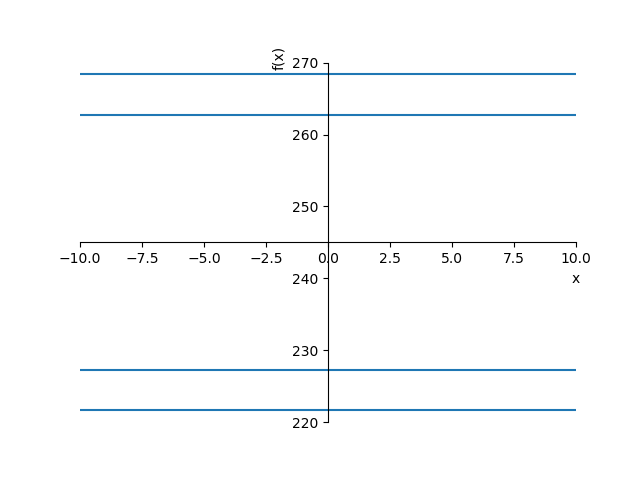
\includegraphics[scale=0.6]{p71e18.png}   \end{solution}\question p71e19- Los pesos de los paquetes de café que envasan en una factoría siguen una distribución normal con un peso
medio de 250 gr y desviación típica de 16 gr. En el proceso de control de calidad del envasado se toma una
muestra de 16 envases cada cuatro horas y se calcula el peso medio de la muestra. Diseña un gráfico sobre el
que podamos representar semanalmente los análisis efectuados y controlar la calidad del proceso con los
niveles de confianza del 95 y 99\%. \begin{solution}   i) Al 95\%: \\  Calculamos el intervalo de confianza para la media, sabiendo que la media muestral es: 250, la desviación típica: 16, tamaño de la muestra: 16 y el grado de confianza: 95.0\%. \\ \\ Valor crítico: \\ $\alpha=1-0.95=0.05\to \frac{\alpha}{2}=0.025$ \\ \\ $P(Z>z_{\alpha/2})=0.025\to P(Z<z_{\alpha/2})=0.975 \to z_{\alpha/2} =1.96$ \\ 
    \begin{tikzpicture}[scale=0.8]
    \pgfmathdeclarefunction{gauss}{2}{\pgfmathparse{1/(#2*sqrt(2*pi))*exp(-((x-#1)^2)/(2*#2^2))}}
    \tikzmath{\conf = 0.95; \crit= 1.96; \a=0.025);}
    \begin{axis}[no markers, domain=-5:5, samples=100, axis lines=left, height=5cm, width=12cm, xtick={0,\crit}, ytick=\empty, xticklabels = {$0$, $z_{\frac{\alpha}{2}}=\crit$},enlargelimits=false, clip=false, axis on top]
      \addplot [fill=cyan!20, draw=none, domain=-\crit:\crit] {gauss(0,1)} \closedcycle;
      \addplot [very thick,cyan!50!black] {gauss(0,1)};
    \end{axis}
    \node[] at (5.2,1.5) {$\conf$};	
    \draw[-]   (\crit+6.5,1)node[right]{$\a$}  --  (\crit+5.6,0.1) ;
    \end{tikzpicture} \\
    Error cometido: \\ $E=z_{\alpha/2}\cdot \frac{\sigma}{\sqrt{n}} \to E=1.96\cdot \frac{16}{4.0}=7.84$ \\ Por tanto el intervalo de confianza será: \\$\left(\overline{x} - E , \overline{x} + E \right)=\left(250 - 7.84 , 250 + 7.84 \right)=\left(242.16, 257.84 \right)$ \\  \\ 
    \begin{tikzpicture}[scale=0.4]
      \tikzmath{\a = -10; \b = 10; \aa = \a -1; \bb = \b + 1 ; \dist = \b - \a; \med = (\a + \b)/2;}
      \draw[very thick] (\a,0) -- (\b,0);
      \path [draw=black, fill=white] (\b,0) circle (2pt);
      \path [draw=black, fill=white] (\a,0.0) circle (2pt);
      \draw[latex-latex] (\a - 1.5,0) -- (\b + 1.5,0) ;
      \draw[shift={(\a,0)},color=black] (0pt,3pt) -- (0pt,-3pt);
      \draw[shift={(\a,0)},color=black] (0pt,0pt) -- (0pt,-3pt) node[below] {$242.16$};
      \draw[shift={(\med,0)},color=black] (0pt,3pt) -- (0pt,-3pt);
      \draw[shift={(\med,0)},color=black] (0pt,0pt) -- (0pt,-3pt) node[below] {$250$};
      \draw[shift={(\b,0)},color=black] (0pt,3pt) -- (0pt,-3pt);
      \draw[shift={(\b,0)},color=black] (0pt,0pt) -- (0pt,-3pt) node[below] {$257.84$};
      \draw[decorate,decoration={brace}, thick](\med,0.2)--(\b,0.2) node[above, midway] {$E=7.84$}; 
    \end{tikzpicture} \\
     \\ ii) Al 99\%: \\  Calculamos el intervalo de confianza para la media, sabiendo que la media muestral es: 250, la desviación típica: 16, tamaño de la muestra: 16 y el grado de confianza: 99.0\%. \\ \\ Valor crítico: \\ $\alpha=1-0.99=0.01\to \frac{\alpha}{2}=0.005$ \\ \\ $P(Z>z_{\alpha/2})=0.005\to P(Z<z_{\alpha/2})=0.995 \to z_{\alpha/2} =2.5758$ \\ 
    \begin{tikzpicture}[scale=0.8]
    \pgfmathdeclarefunction{gauss}{2}{\pgfmathparse{1/(#2*sqrt(2*pi))*exp(-((x-#1)^2)/(2*#2^2))}}
    \tikzmath{\conf = 0.99; \crit= 2.5758; \a=0.005);}
    \begin{axis}[no markers, domain=-5:5, samples=100, axis lines=left, height=5cm, width=12cm, xtick={0,\crit}, ytick=\empty, xticklabels = {$0$, $z_{\frac{\alpha}{2}}=\crit$},enlargelimits=false, clip=false, axis on top]
      \addplot [fill=cyan!20, draw=none, domain=-\crit:\crit] {gauss(0,1)} \closedcycle;
      \addplot [very thick,cyan!50!black] {gauss(0,1)};
    \end{axis}
    \node[] at (5.2,1.5) {$\conf$};	
    \draw[-]   (\crit+6.5,1)node[right]{$\a$}  --  (\crit+5.6,0.1) ;
    \end{tikzpicture} \\
    Error cometido: \\ $E=z_{\alpha/2}\cdot \frac{\sigma}{\sqrt{n}} \to E=2.5758\cdot \frac{16}{4.0}=10.3032$ \\ Por tanto el intervalo de confianza será: \\$\left(\overline{x} - E , \overline{x} + E \right)=\left(250 - 10.3032 , 250 + 10.3032 \right)=\left(239.6968, 260.3032 \right)$ \\  \\ 
    \begin{tikzpicture}[scale=0.4]
      \tikzmath{\a = -10; \b = 10; \aa = \a -1; \bb = \b + 1 ; \dist = \b - \a; \med = (\a + \b)/2;}
      \draw[very thick] (\a,0) -- (\b,0);
      \path [draw=black, fill=white] (\b,0) circle (2pt);
      \path [draw=black, fill=white] (\a,0.0) circle (2pt);
      \draw[latex-latex] (\a - 1.5,0) -- (\b + 1.5,0) ;
      \draw[shift={(\a,0)},color=black] (0pt,3pt) -- (0pt,-3pt);
      \draw[shift={(\a,0)},color=black] (0pt,0pt) -- (0pt,-3pt) node[below] {$239.6968$};
      \draw[shift={(\med,0)},color=black] (0pt,3pt) -- (0pt,-3pt);
      \draw[shift={(\med,0)},color=black] (0pt,0pt) -- (0pt,-3pt) node[below] {$250$};
      \draw[shift={(\b,0)},color=black] (0pt,3pt) -- (0pt,-3pt);
      \draw[shift={(\b,0)},color=black] (0pt,0pt) -- (0pt,-3pt) node[below] {$260.3032$};
      \draw[decorate,decoration={brace}, thick](\med,0.2)--(\b,0.2) node[above, midway] {$E=10.3032$}; 
    \end{tikzpicture} \\
    Por tanto el gráfico de control quedará: \\ 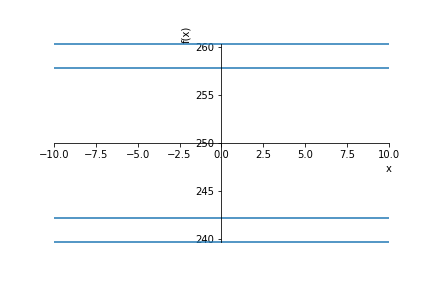
\includegraphics[scale=0.6]{p71e19.png}   \end{solution}
    \end{questions}
    \end{document}
    